\section{Detector Calibration and Alignment}
\label{sec:calibration}

The calibration and alignment parameters needed by the reconstruction algorithms reside in the conditions database described below, along with the metadata allowing for versioning and defining the run/subrun range over which any set of calibration constants are valid. Several concurrent sets of calibrations will cover different use cases, for example, an initial set of values used during reconstruction for the trigger. Nominally, a given calibration set can be extended with values covering a new set of runs, allowing calibrated reconstruction to be performed on those runs. When calibration algorithms are updated or inputs are changed, a new version of the calibration set can be defined as well, possibly requiring reprocessing of relevant runs. The calibrations can also be overridden with text files, so iterating calibration procedures can easily include rerunning reconstruction using the previous step's results.

A large part of the calibration and alignment will be performed in situ, using cosmic ray or beam data collected during normal (including extracted position) Mu2e running conditions. There are also several sources of calibration data that will need dedicated setup and runs, including tracker charge injection pulsers, calorimeter laser system and DT source, Y-88 and Eu-152 sources for the stopping target monitor, etc. Most of these will also require specialized data processing. The various detector alignment procedures will also make use of metrology measurements made during both construction and after installation.

\subsection{Tracker calibration}

The majority of the tracker calibrations will be performed iteratively using data from reconstructed extracted or off-spill cosmic tracks. For extracted cosmics, the initial triggering and event selection is based on a simple time clustering of hits in the tracker. Each cluster is then reconstructed using both a KinKal Kalman filter track fit as well as a maximum likelihood-based straight-line track fit. Both track fit results are processed with Mu2e Offline modules to produce simplified output for calibration. 

Information from the KinKal fit is used to determine tracker calibration parameters from the TrkAna trees, including channel time offsets, time-to-distance relationships, and the TOT-to-drift time. Mean residuals for each channel are used to calculate corrections to the calibrations. Collecting a few thousand hits per channel requires around one day of extracted cosmic data.

The likelihood fit results are used to align the tracker modules with the Millepede-II algorithm~\cite{millepede1,millepede2}. Given a set of track fits Millepede-II performs a simultaneous least squares fit to all track parameters and alignment parameters, including correlations. It can be run interactively, taking only a few minutes to process millions of tracks. The Millepede fit can also include results from metrology measurements as Gaussian constraints on any linear combination of the alignment parameters. Separate 6-DOF alignment parameters are included for different levels of tracker modules, including each panel, plane, and the entire tracker. Redundant degrees of freedom are removed by applying fixed constraints within Millepede. We plan to eventually use KinKal fits of off-spill cosmic tracks for alignment as well, which should provide better constraints on systematic shifts and rotations. A track refit based on General Broken Lines~\cite{gbl} would allow us to reformulate the KinKal result and use Millepede again. 

Both the alignment and calibration are performed iteratively. Each iteration requires re-performing the hit and track reconstruction on the uncalibrated digi and producing a new set of data, but we expect the number of iterations to be small, even for initial bootstrapping. After convergence, the updated calibration and alignment parameters are uploaded to the condition database, and the calibration set can be extended to include new values to allow for pass-2 reconstruction. 

The ability to bootstrap the calibration and alignment using the first cosmic data was demonstrated using simulations. In the simulations, calibration and alignment parameters are set to randomly distributed values to model uncalibrated reconstruction. Additionally, parameters for the detector configuration like thresholds and channel statuses are varied. Simulations of cosmic data in the extracted position were produced using distributions of calibration parameters and states that model the expected condition of the detector for the initial data taking. The KinKal track fit with a reduced set of annealing steps is used for the first iteration of the calibration, after which the likelihood fit and full KinKal fit can be used for further steps. The performance of the calibrated track reconstruction is shown in Figure~\ref{fig:calibLong}. 


\begin{figure}[tbp]
  \centering
  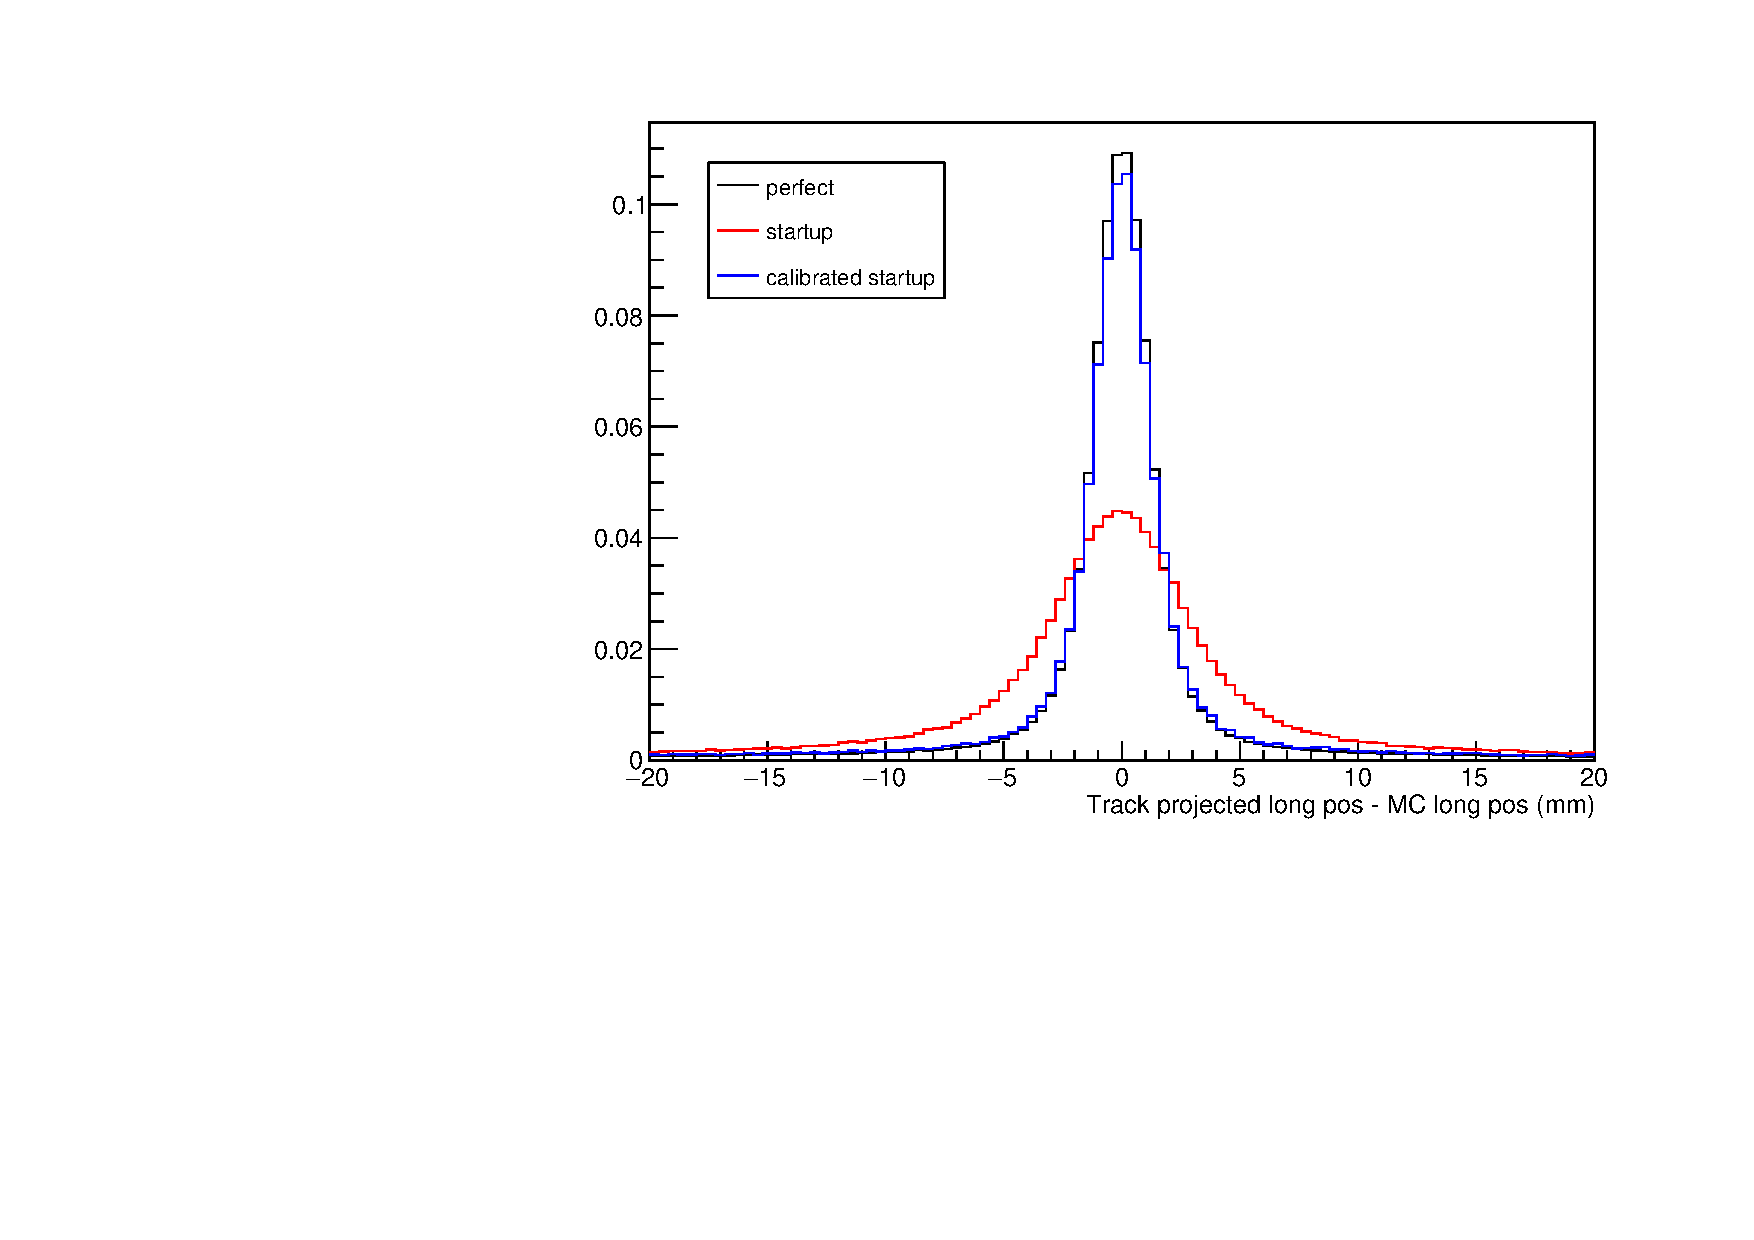
\includegraphics[height=0.4\textwidth]{figures/calibratedlong.pdf}%
  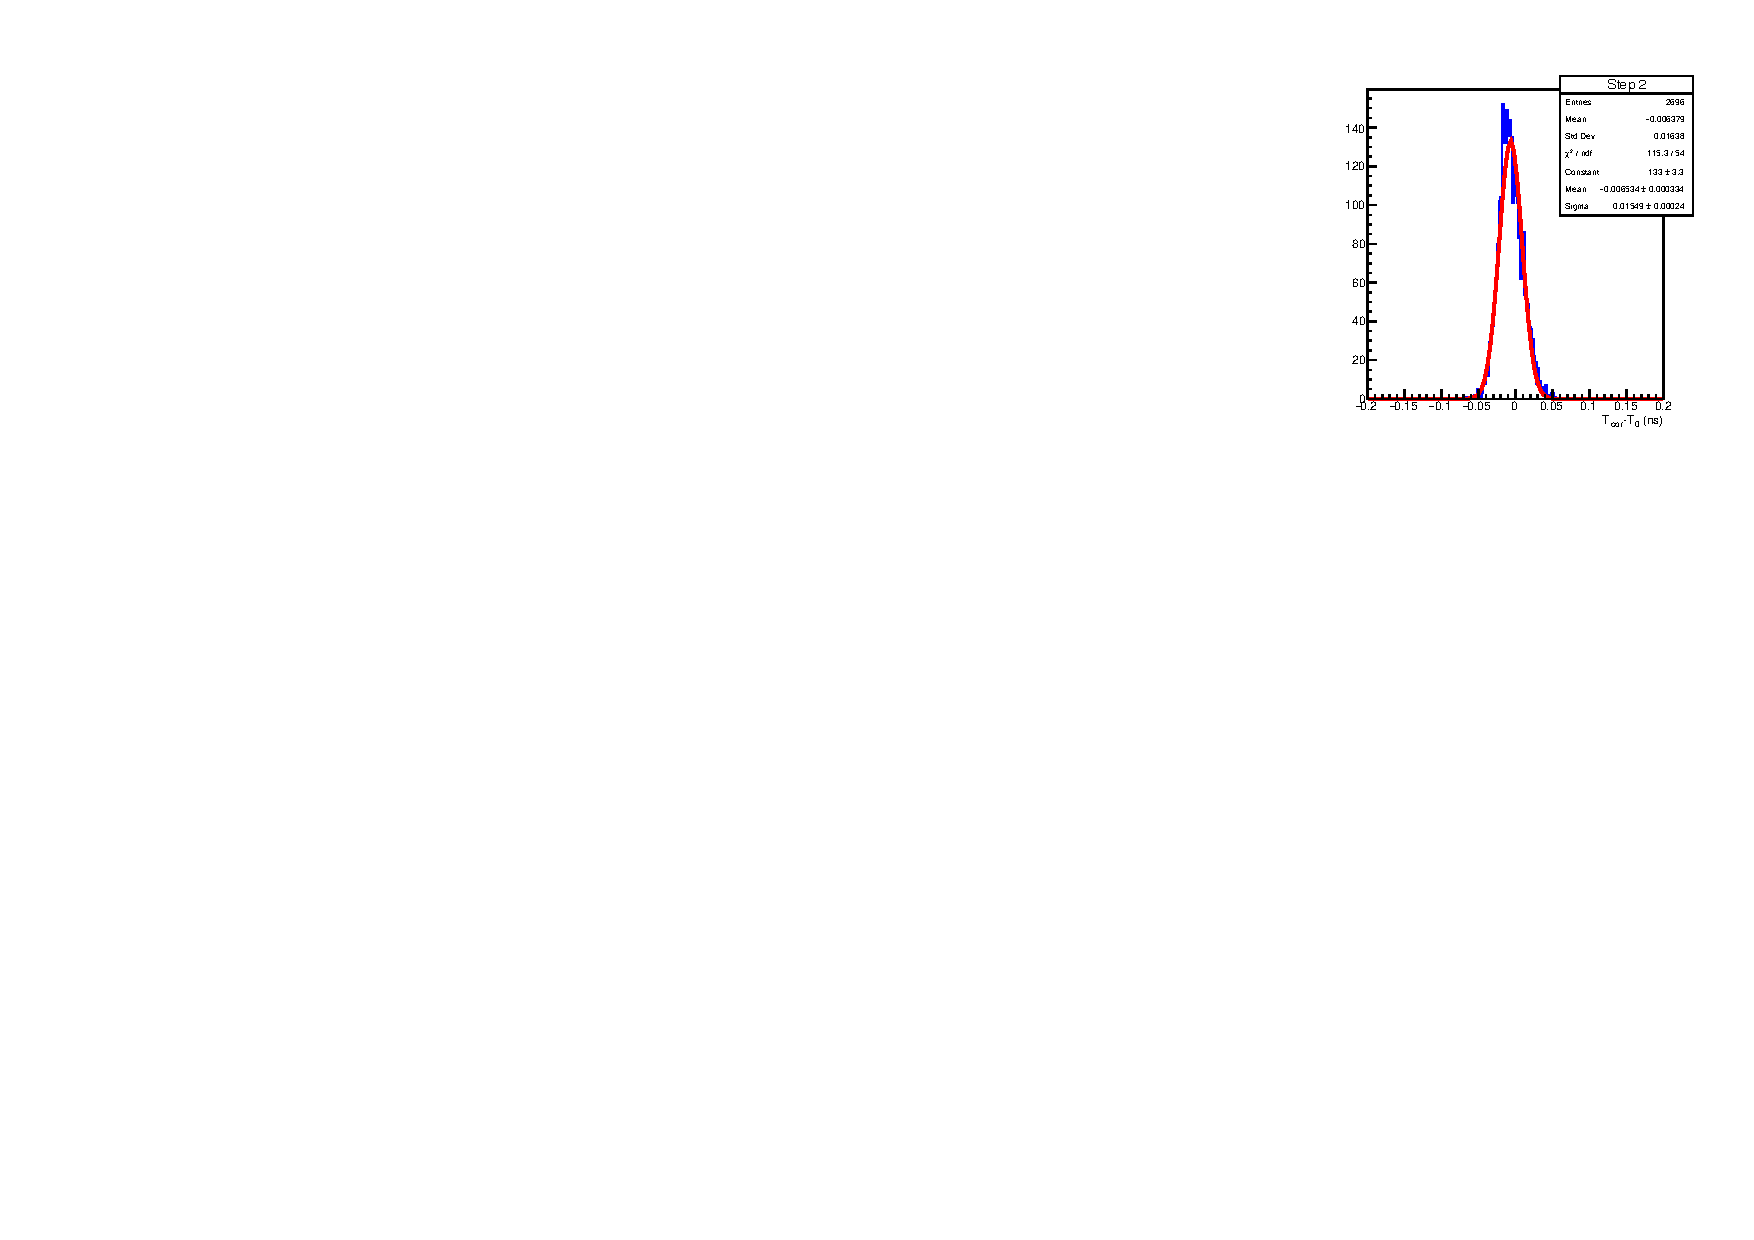
\includegraphics[height=0.4\textwidth]{figures/caloCalibTime.pdf}
  \caption{Left: Track fit longitudinal resolution in uncalibrated and calibrated simulated startup condition data as well as perfect simulated data. Right: Results of the calorimeter energy calibration procedure based on a simulated sample of cosmic rays equivalent to a data-taking period of 10 hours.}
  \label{fig:calibLong}
\end{figure}


\subsection{Calorimeter calibration}

The calorimeter makes use of three different calibration methods, based on the laser system, the source calibration systems, and cosmic ray events.

Cosmics calibration requires data samples in extracted position or off-spill during physics runs. The energy calibration is performed with minimum ionizing particles, identified as events with clusters from straight tracks with a minimum energy deposit. A $\sim 0.5\%$ spread is obtained from 10-hour simulated cosmic ray events in extracted position. The time calibration is performed in two steps. First, reconstructed hits produced by the laser are used to evaluate time offsets due to the electronics. The second step performs a least squares fit to clusters produced by minimum ionizing particles to calculate a correction to the time offsets for each channel. Simulation studies show that 15 ps time alignment is obtained. The energy and time calibration procedures have been validated using data collected by a large-scale calorimeter prototype containing 52 crystals. Results are consistent with MC expectations, demonstrating the robustness of the procedures.

The calorimeter has a radioactive source-based calibration system that allows for an absolute energy calibration of each crystal using a 6.13 MeV photon line. The distribution of reconstructed energy for each crystal is fit with 3 crystal ball functions - for the main peak and two escape peaks - over a logistic background. This calibration has been tested using simulations that include crystal non-uniformity, electronics noise, and different photo-statistics, demonstrating consistency to less than one percent with data from a ten-minute long run. The laser system distributes green light to each calorimeter SiPM to perform a precise gain determination, with a dedicated run of a few minutes, and monitor the stability of the response by continuously firing a few pulses in the off-spill data collection period. Source and laser runs will be performed on a weekly basis.

The results from each calibration source are stored in "archive'' tables in the condition database (see Section~\ref{sec:databases}), and combined to produce the final calibration constants stored in the condition database. 

The calorimeter alignment is determined during construction using a laser tracker survey with a $\mathcal{O}(100\ \mu \text{m})$ accuracy on crystal position, enough for calorimeter reconstruction purposes. The geometrical alignment of the calorimeter will be completed once on the Mu2e detector train, through three aiming points placed on the calorimeter external structure. Cosmic ray events will then be used to determine the position and time alignment with respect to the tracker and the CRV.

\subsection{CRV calibration}

The CRV uses a special set of non-zero-suppressed waveforms for calibration, collected and digitized alongside normal data taking. The first stage processes the raw CRV digis and histograms the waveform values to calculate per channel pedestal values. Once pedestals have been calibrated, pulse reconstruction can be run, and an Offline module aggregates pulse heights and areas for dark rate pulses. A standalone script then fits for the single PE value for each channel.

This pulse calibration includes temperature corrections and requires data read out by the slow controls, both in the calibration process and in the calibrated pulse reconstruction. Initially, these temperatures are stored in a separate slow control database and are then imported into the reconstruction's conditions database at regular intervals (once every hour, depending on the temperature fluctuations in the Mu2e hall). Less than one second of non-zero-suppressed data is required for the full CRV pulse calibration.

Reconstruction and calibration of dark pulses from the non-zero-suppressed waveforms takes around 0.5 seconds per microbunch, or about 7 hours for the full pulse calibration dataset. These procedures have been demonstrated on data from several test stands so far.

%\begin{figure}[tbp]
%  \centering
%  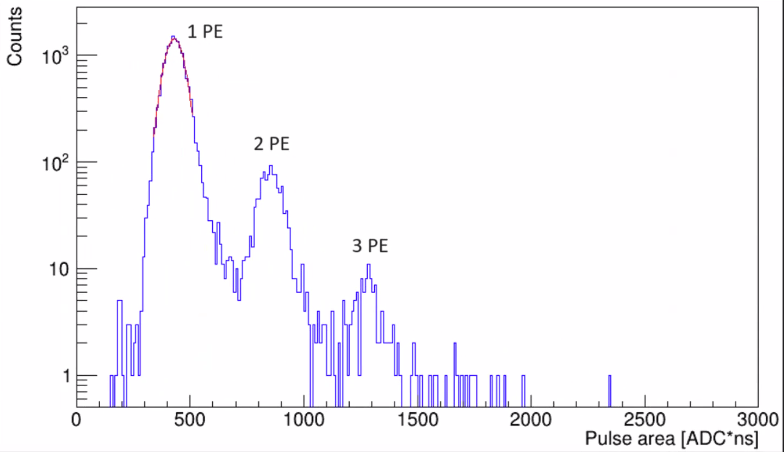
\includegraphics[width=0.5\textwidth]{figures/crvpulsefit.png}%
%  \caption{Output from CRV pulse reco from teststand data used to calibrate %pulse shapes. Single and multiple pe peaks are clearly seen.
%  }%
%  \label{fig:crvpulse}
%\end{figure}


\subsection{STM calibration}
The location of the STM and its collimation system is initially performed by optical survey. The relative alignment of the upstream and downstream structures will be then monitored by a laser alignment system to ensure that there are no large changes in the alignment that need to be corrected.

Acceptance and energy scale will be calibrated using Eu-152 and Y-88 sources. During data taking, the energy scale is expected to be stable over a few hours. Beam data will be used to monitor energy scale drift using various spectra lines (x-ray, gamma ray, 511 keV). Calibration constants will be stored in the conditions database. The time delay between the STM detectors and the other detectors can be measured using a scintillator paddle with a known cable length.

%\subsection{Extinction monitor calibration}